% ══════════════════════════════════════════════════════════════════
% COVER PAGE
% ══════════════════════════════════════════════════════════════════
% --- Page Réseaux ou autre PDF
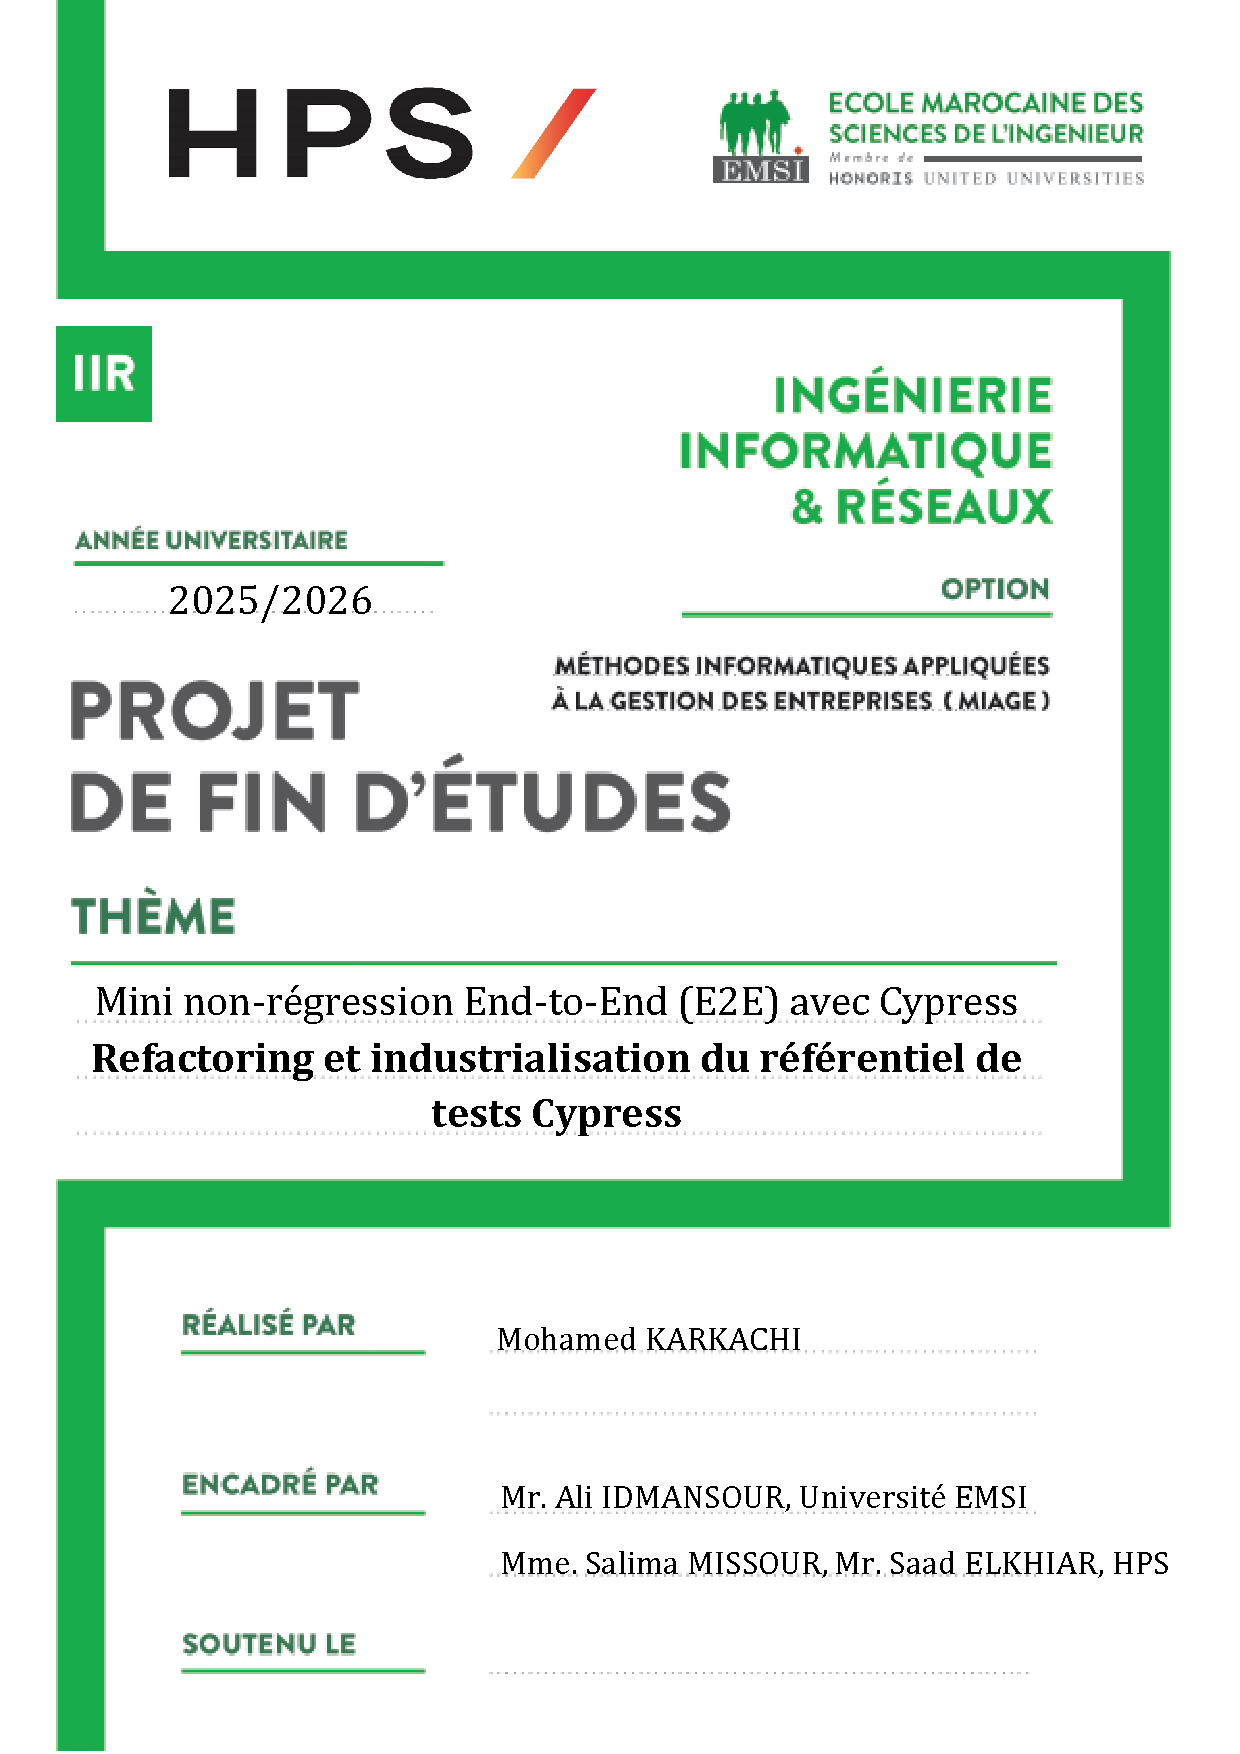
\includepdf{IIR.pdf}

% ══════════════════════════════════════════════════════════════════
% DÉDICACE
% ══════════════════════════════════════════════════════════════════
\newpage
\chapter*{Dédicace}
\addcontentsline{toc}{chapter}{Dédicace}

\begin{center}
\fontsize{16}{19}\itshape\selectfont
À mes chers parents,\\
pour tous leurs sacrifices, leur amour, leur tendresse, leur soutien et leurs prières tout au long de mes études.\\
À ma chère famille, pour leur encouragement permanent.\\
À mes professeurs et amis, pour leur aide et leur soutien.\\
Je vous dédie ce travail.
\end{center}

% ══════════════════════════════════════════════════════════════════
% REMERCIEMENTS
% ══════════════════════════════════════════════════════════════════
\newpage
\chapter*{Remerciements}
\addcontentsline{toc}{chapter}{Remerciements}

\begin{center}
\fontsize{16}{19}\itshape\selectfont
Je tiens tout d'abord à remercier Madame Salima MISSOUR, mon encadrante de stage pour son suivi et son accompagnement tout au long de ce stage, ainsi que Madame Meryem Fouzair de m'avoir accueilli dans le premier jour de mon stage.\\[10pt]

Mes remerciements vont également à Monsieur Fabrice Soto et Jérôme PEIGNIEN, pour leurs encadrements techniques qui m'a permis de monter en compétences sur différents sujets et pour leurs présences et leurs disponibilités.\\[10pt]

Je tiens également à exprimer ma gratitude à l'ensemble de l'équipe de tests, de m'avoir accueilli, accompagné et pris de temps de répondre à mes questions.\\[10pt]

Je tiens également à exprimer ma reconnaissance à Mr. Ali IDMANSOUR pour avoir supervisé mon stage, pour ses remarques et ses conseils. Mes remerciements vont aussi à l'ensemble du corps professoral de l'université EMSI pour leurs efforts afin de réussir cette année exceptionnelle.\\[10pt]

Enfin, un chaleureux remerciement à ma famille, particulièrement, mes parents qui m'ont apporté, sans réserve, tout le soutien et l'affection nécessaires pour le bon déroulement de mon stage.
\end{center}

% ══════════════════════════════════════════════════════════════════
% RÉSUMÉ
% ══════════════════════════════════════════════════════════════════
\newpage
\chapter*{Résumé}
\addcontentsline{toc}{chapter}{Résumé}

{\fontsize{14}{17}\selectfont
Ce présent document résume tous les travaux effectués pendant mon stage PFE, qui s'intitule « Automatisation des tests », au titre du projet de fin d'études.

L'automatisation des tests est un moyen qui est de plus en plus apprécié par les organisations. Elle se présente comme une solution efficace permettant d'éviter les erreurs humaines lors de la répétition d'exécution des tests et gagner du temps. D'où l'idée d'intégrer une équipe d'automatisation de test du groupe HPS qui compte parmi les grands éditeurs de logiciel monétique. Ma mission durant ce stage est l'automatisation des tests de quelques fonctionnalités de la solution monétique d'HPS.

Pour aboutir à mes fins et accomplir ma mission, il a été indispensable de suivre un ensemble d'étapes : en commençant par les formations puis définition de l'environnement de test, l'analyse des cahiers de spécification technique, la conception des tests et des jeux de données, l'implémentation des scénarios de test, l'exécution manuellement des tests avant de les automatisés et enfin la rédaction du rapport au fur et à mesure de la réalisation de la mission.

Au-delà de l'automatisation classique, ce projet introduit une approche innovante : le développement d'un \textbf{QA Cypress Generator Dashboard}, une plateforme full-stack alimentée par l'\textbf{IA (Mistral)} et l'\textbf{orchestration de workflows (n8n)}, permettant aux testeurs QA de générer, exécuter et surveiller des scripts de tests Cypress E2E sans écrire une seule ligne de code.

\vspace{10pt}
\textbf{Mots clés :} Automatisation des tests, Cypress, React, Node.js, PowerCARD, Assurance Qualité, IA, n8n, Microservices
}

% ══════════════════════════════════════════════════════════════════
% GLOSSAIRE
% ══════════════════════════════════════════════════════════════════
\newpage
\chapter*{Glossaire}
\addcontentsline{toc}{chapter}{Glossaire}

{\fontsize{14}{17}\selectfont
\begin{description}[leftmargin=3cm,style=nextline]
\item[AI] Artificial Intelligence (Intelligence Artificielle)
\item[API] Application Programming Interface
\item[ATM] Automated Teller Machine
\item[BRD] Business Requirement Description
\item[BSD] Business Solution Description
\item[DB] Data Base
\item[E2E] End-To-End (Test de bout en bout)
\item[EMSI] Ecole Marocaine des Sciences de l'Ingénieur
\item[FTP] File Transfer Protocole
\item[FTPS] File Transfer Protocole Secure
\item[HPS] Hightech Payment Systems
\item[HSBC] Hong-Kong and Shanghai Banking Corporation
\item[ISTQB] International Software Testing Qualifications Board
\item[JEE] Java Entreprise Edition
\item[JSF] Java Server Faces
\item[JWT] JSON Web Token
\item[LLM] Large Language Model
\item[MCP] Model Context Protocol
\item[n8n] Outil d'automatisation de workflows open-source
\item[PTT] PowerTools Tests
\item[PWC] PowerCARD
\item[QA] Quality Assurance (Assurance Qualité)
\item[REST] Representational State Transfer
\item[SFTP] SSH File Transfer Protocol
\item[SPA] Single Page Application
\item[SQL] Structured Query Language
\item[SSE] Server-Sent Events
\item[UI] User Interface
\item[UNIX] Unix
\item[WS] Web Service
\item[XML] Extensible Markup Language
\end{description}
}

% ══════════════════════════════════════════════════════════════════
% TABLE DES MATIÈRES
% ══════════════════════════════════════════════════════════════════
\newpage
\tableofcontents

% ══════════════════════════════════════════════════════════════════
% LISTE DES FIGURES ET TABLEAUX
% ══════════════════════════════════════════════════════════════════
\newpage
\listoffigures
\newpage
\listoftables
